%
% $RCSfile: computer_hardware.tex,v $
%
% Copyright (C) 2002-2008. Christian Heller.
%
% Permission is granted to copy, distribute and/or modify this document
% under the terms of the GNU Free Documentation License, Version 1.1 or
% any later version published by the Free Software Foundation; with no
% Invariant Sections, with no Front-Cover Texts and with no Back-Cover
% Texts. A copy of the license is included in the section entitled
% "GNU Free Documentation License".
%
% http://www.cybop.net
% - Cybernetics Oriented Programming -
%
% http://www.resmedicinae.org
% - Information in Medicine -
%
% Version: $Revision: 1.1 $ $Date: 2008-08-19 20:41:06 $ $Author: christian $
% Authors: Christian Heller <christian.heller@tuxtax.de>
%

\subsubsection{Computer Hardware}
\label{computer_hardware_heading}
\index{Computer Hardware}
\index{Human Being}
\index{Technical Environment}
\index{Biological Environment}

Gilbert Carl Herschberger II writes \cite{josgeneral}: \textit{A computer is a
grossly oversimplified model of a human being. Humans can learn more about
themselves by working with this model. And, they might learn more about what
makes a good model by looking at themselves.} To the many analogies a computer
has with a human being belong its input/ output (i/o) devices (figure
\ref{computer_figure}), many of which have an equivalent organ in the human
body:

\begin{itemize}
    \item[-] \emph{Eye}: Camera, Scanner
    \item[-] \emph{Ear}: Microphone
    \item[-] \emph{Nose, Tongue}: Sensors
    \item[-] \emph{Skin}: Keyboard, Mouse, Joystick
    \item[-] \emph{Larynx}: Loudspeaker
    \item[-] \emph{Extremity}: Monitor, Printer, Braille Panel, Arm, Wheel
\end{itemize}

\begin{figure}[ht]
    \begin{center}
        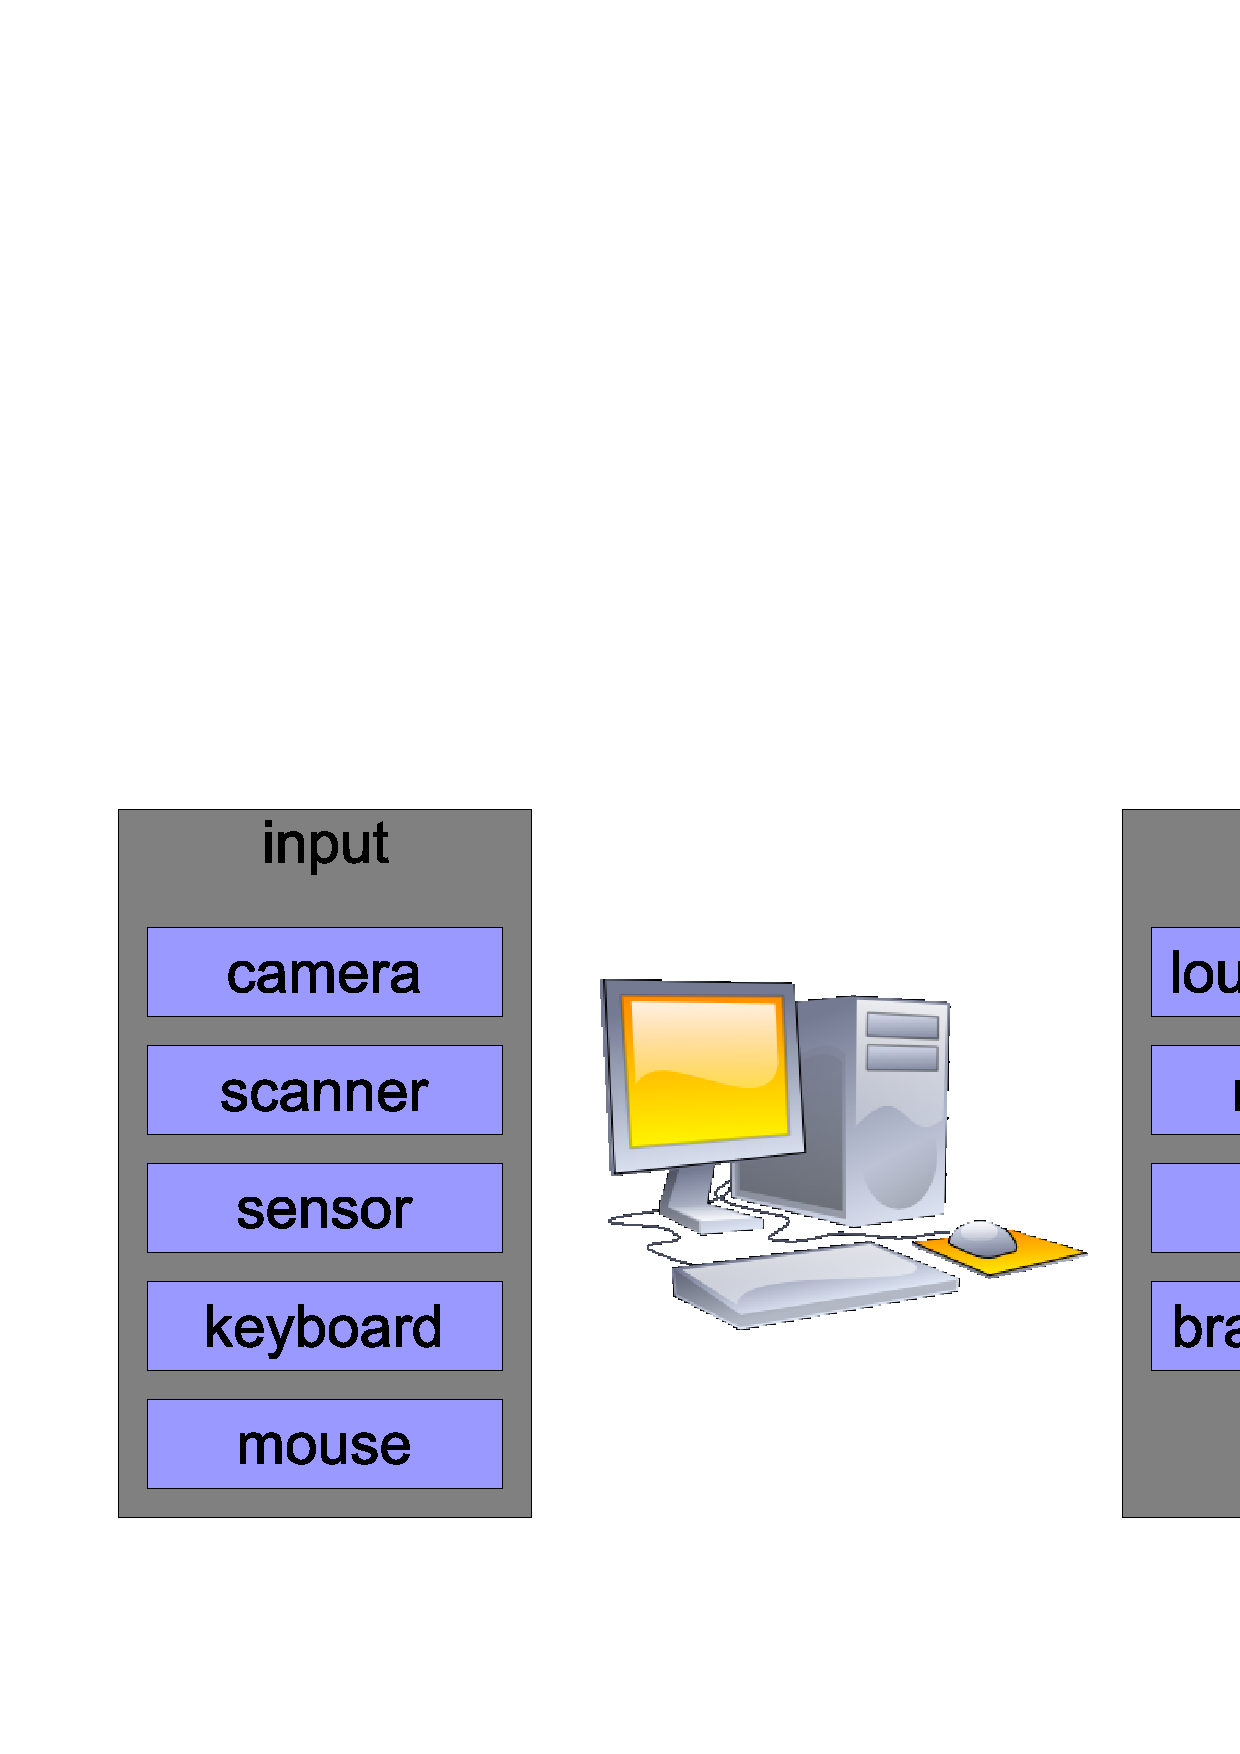
\includegraphics[scale=0.3,angle=-90]{graphic/computer.pdf}
        \caption{Computer Hardware with Input- and Output Devices}
        \label{computer_figure}
    \end{center}
\end{figure}

The difference to \emph{Robotics} is that a robot has additional devices.
Various \emph{Sensors} are used for information input; many moveable parts like
\emph{Arms} or \emph{Wheels} take motoric action and can be compared to the
extremities of the human body. Table \ref{environment_table} gives an
impression of how technical and biological environments can be compared.

\begin{figure}[ht]
    \begin{center}
        \begin{footnotesize}
        \begin{tabular}{| p{25mm} | p{50mm} | p{30mm} |}
            \hline
            \textbf{Ontological Level} & \textbf{Technical System} & \textbf{Biological Equivalent}\\
            \hline
            Network & Internet, Wide Area Network (WAN) & Society, Biotope\\
            \hline
            Family & Local Area Network (LAN) & Family\\
            \hline
            System & Computer & Organism\\
            \hline
            Block & Component & Organ\\
            \hline
        \end{tabular}
        \end{footnotesize}
        \caption{Ontology comparing Technical- and Biological Environment}
        \label{environment_table}
    \end{center}
\end{figure}

To sum up: Among the abstract knowledge models stored in a system are some that
describe the structure and capabilities of the system itself.
